\documentclass[12pt, twoside]{article}
\usepackage[letterpaper, margin=1in, headsep=0.5in]{geometry}
\usepackage[english]{babel}
\usepackage[utf8]{inputenc}
\usepackage{amsmath}
\usepackage{amsfonts}
\usepackage{amssymb}
\usepackage{tikz}
%\usetikzlibrary{quotes, angles}

\usepackage{graphicx}
\usepackage{enumitem}
\usepackage{multicol}

\usepackage{fancyhdr}
\pagestyle{fancy}
\fancyhf{}
\renewcommand{\headrulewidth}{0pt} % disable the underline of the header

\fancyhead[RE]{\thepage}
\fancyhead[RO]{\thepage \\ Name: \hspace{3cm}}
\fancyhead[L]{BECA / Dr. Huson / 10th Grade Geometry\\* 11 April 2019}

\begin{document}
\subsubsection*{9-11 Homework: Similar triangles, dilation ratios review}
 \begin{enumerate}

  \begin{multicols}{2}
  [\item A dilation maps triangle $PQR$ onto triangle $STU$ with $QR=5$ and $TU=7.5$.] \vspace{0.75cm}
    \begin{enumerate}
      \item $\overline{QR} \rightarrow$ \rule{2cm}{0.15mm}
      \item Complete the fraction numerators with the corresponding segment and length: \\[0.75cm]
      $\displaystyle k=\frac{\qquad}{QR} =\frac{\qquad}{5}$
      \item What scale factor maps\\
       $\triangle PQR \rightarrow \triangle STU$?
    \end{enumerate}
    \begin{tikzpicture}[scale=0.9]
      \coordinate [label=above left:$P$](A) at (85:2);
      \coordinate [label=below:$Q$](B) at (0, 0);
      \coordinate [label=right:$R$](C) at (-20:3);
      \draw [thick] (A)--(B)--(C)--cycle;

      \draw [thick, xshift=2cm, yshift=2.5cm] (85:3) node[above]{$S$}--
      (0,0) node[below]{$T$}--
      (-20:4.5) node[right]{$U$}--cycle;
    \end{tikzpicture}
  \end{multicols}  \vspace{1cm}

 \item Triangle $ABC$ is dilated with a scale factor of $k$ centered at $A$, yielding $\triangle ADE$, as shown. Given $AB=9$, $BC=12$, $AC=15$, and $DE=16$. \\[0.25cm] Find $BD$, $AE$, and $k$ (the scale factor). \vspace{0.5cm}
 \begin{center}
     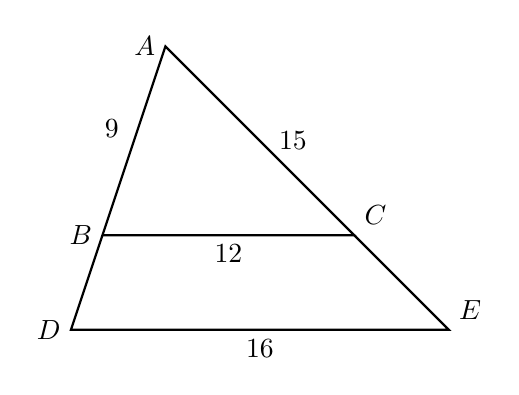
\begin{tikzpicture}[scale=0.4]
       \draw [thick]
       (0,0)node[left]{$B$}--
       (8,0)node[above right]{$C$}--
       (2,6)node[left]{$A$}--cycle;
       \draw [thick]
       (0,0)--
       (-1,-3)node[left]{$D$}--
       (11,-3)node[above right]{$E$}--(8,0);
       \node at (4,0)[below]{$12$};
       \node at (5.3, 3)[right]{$15$};
       \node at (0.3, 2.8)[above]{$9$};
       \node at (5,-3)[below]{$16$};
     \end{tikzpicture}
   \end{center}
\vspace{2cm}

 \item Given $\triangle JKL \sim \triangle MNO$. $m\angle J = 48^\circ$ and $m\angle L = 87^\circ$.\\
 Find the measure of $\angle N$.

\newpage

\begin{multicols}{2}[\item The diagram below shows $\triangle ABC$, with $\overline{AEB}$, $\overline{ADC}$, and $\angle ACB \cong \angle AED$. $AB=8$, $AD=4$, and $DE=2$.]
    \begin{enumerate}
      \item $\triangle ADE \rightarrow$ \rule{2cm}{0.15mm} \vspace{1cm}
      \item $\overline{AD} \rightarrow$ \rule{2cm}{0.15mm} \vspace{1cm}
      \item What is the scale factor?\\[0.5cm] $k=$  \rule{2cm}{0.15mm}
      \item What is the length of $\overline{BC}$?
    \end{enumerate}
     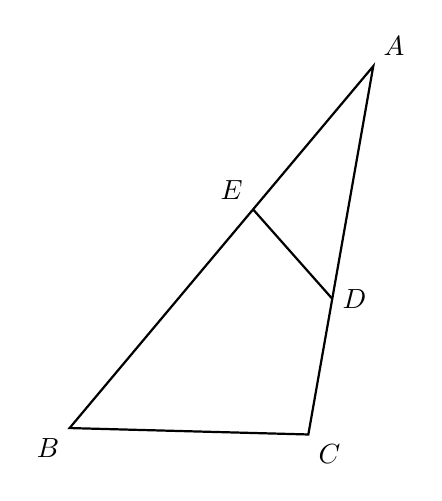
\begin{tikzpicture}%[scale=.48]
       \draw [thick]
       (0,0) node[above right] {$A$}--
       (230:6) node[below left] {$B$}--
       (260:4.75) node[below right] {$C$}--cycle;
       \draw [thick]
       (230:2.375) node[above left] {$E$}--
       (260:3) node[right] {$D$}--cycle;
     \end{tikzpicture}
   \end{multicols} \vspace{2cm}

 \begin{multicols}{2} [\item Circle YES or NO to indicate whether the given transformation maps the hexagon $ABCDEF$ onto itself.]
 \vspace{0.5cm}
  \begin{enumerate}
    \item Yes \quad No \quad A rotation of $120^\circ$ counterclockwise around its center.
     \item Yes \quad No \quad A reflection over $\overleftrightarrow{AD}$
     \item Yes \quad No \quad A reflection over a line through the midpoints of  $\overline{BC}$ and $\overline{EF}$.
     \item Yes \quad No \quad A rotation of $60^\circ$ clockwise around $A$.
     \end{enumerate}
   \begin{center}
       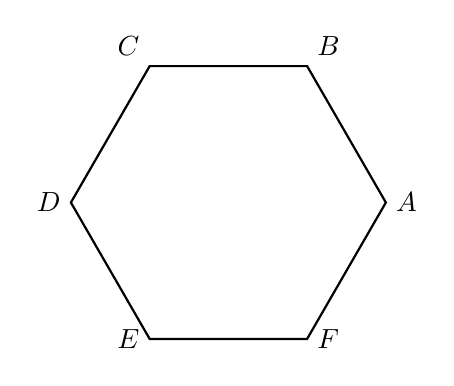
\begin{tikzpicture}%[scale=.48]
         \draw [thick]
         (0:2) node[right] {$A$}--
         (60:2) node[above right] {$B$}--
         (120:2) node[above left] {$C$} --
         (180:2) node[left] {$D$}--
         (240:2) node[left] {$E$}--
         (300:2) node[right] {$F$}--cycle;
       \end{tikzpicture}
     \end{center}
   \end{multicols} \vspace{0.5cm}

   \item What is the length of the segment $A(-2,1)$, $B(3,13)$?

  \end{enumerate}
  \newpage
\subsubsection*{8-10 Homework: Pretest on similar triangles, dilation, \& symmetry}
 \begin{enumerate}

  \item What series of transformations map $\triangle ABC$ onto $\triangle DEF$, shown below? Fully specify the transformations.
    \begin{center}
      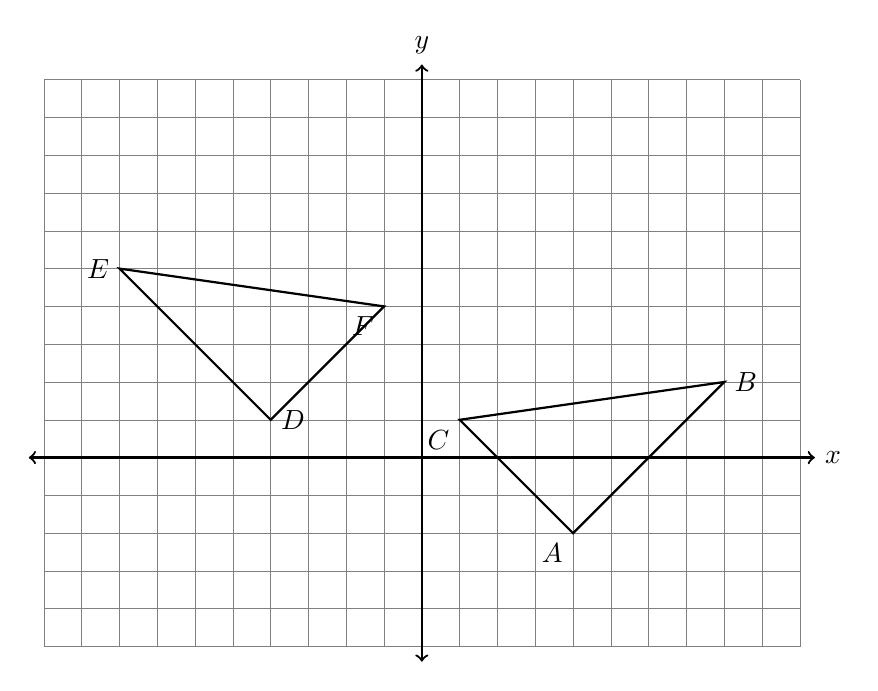
\begin{tikzpicture}[scale=.48]
        \draw [help lines] (-10,-5) grid (10,10);
        \draw [thick, <->] (-10.4,0) -- (10.4,0) node [right] {$x$};
        \draw [thick, <->] (0,-5.4)--(0,10.4) node [above] {$y$};
        \draw [thick]
          (4,-2) node[below left] {$A$}--
          (8,2) node[right] {$B$}--
          (1,1) node[below left] {$C$}--cycle;
        \draw [thick]
          (-4,1) node[right] {$D$}--
          (-8,5) node[left] {$E$}--
          (-1,4) node[below left] {$F$}--cycle;
      \end{tikzpicture}
    \end{center}
\vspace{2cm}

 \item Given $\triangle ABP$ and $\triangle JKP$ as shown below. $\overline{AB} \parallel \overline{JK}$. $AP=10$, $JP=18$, and $JK=27$. Find $AB$.
 \begin{center}
   \begin{tikzpicture}[scale=1.4]
       \draw [thick]
         (0.25,-1)node[right]{$B$}--
         (-0.5,2)node[left]{$K$}--
         (4,0)node[right]{$J$}--
         (0,0)node[above right]{$P$}--
         (-2,0)node[left]{$A$}--cycle;
     \end{tikzpicture}
     \end{center}
 \vspace{2cm}

\newpage
 \item Triangle $ABC$ is dilated with a factor of $\frac{3}{2}$ centered at $A$, yielding $\triangle ADE$, as shown. Given $AB=8$, $BC=12$, and $AC=14$. \\[0.25cm] Find $BD$, $AE$, and $DE$. \vspace{1cm}
 \begin{center}
     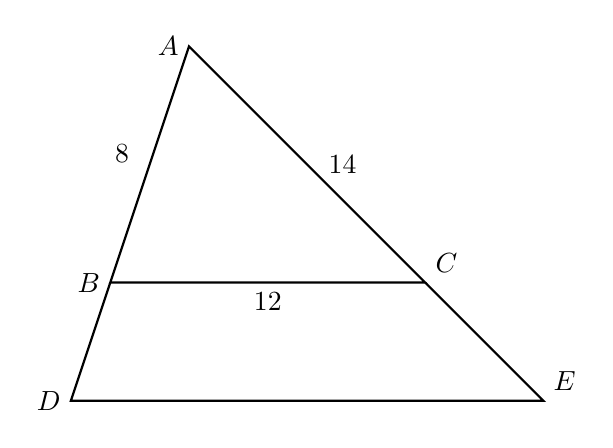
\begin{tikzpicture}[scale=0.5]
       \draw [thick]
       (0,0)node[left]{$B$}--
       (8,0)node[above right]{$C$}--
       (2,6)node[left]{$A$}--cycle;
       \draw [thick]
       (0,0)--
       (-1,-3)node[left]{$D$}--
       (11,-3)node[above right]{$E$}--(8,0);
       \node at (4,0)[below]{$12$};
       \node at (5.3, 3)[right]{$14$};
       \node at (0.3, 2.8)[above]{$8$};
     \end{tikzpicture}
   \end{center}


   \item The grid shows $\triangle ABC$ and $\triangle DEF$.
     \begin{center}
       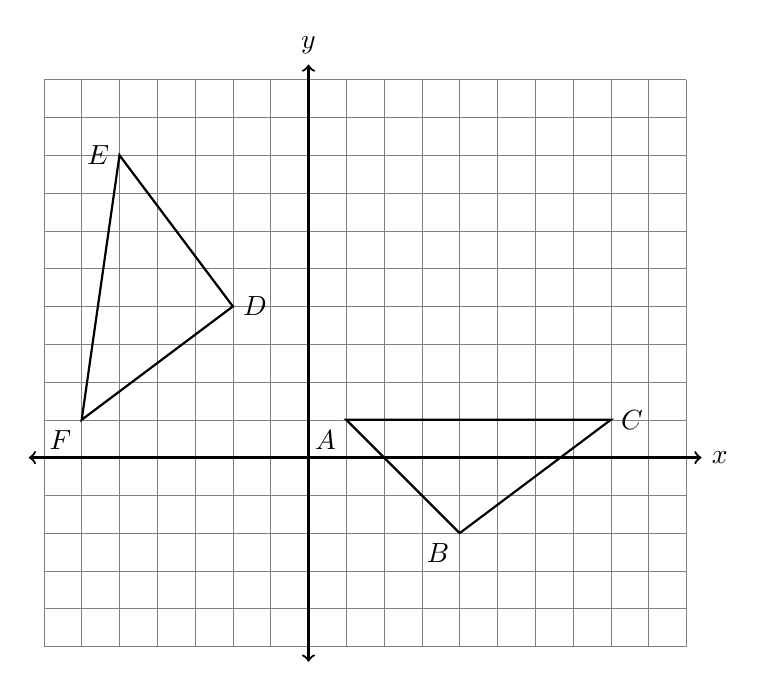
\begin{tikzpicture}[scale=.48]
         \draw [help lines] (-7,-5) grid (10,10);
         \draw [thick, <->] (-7.4,0) -- (10.4,0) node [right] {$x$};
         \draw [thick, <->] (0,-5.4)--(0,10.4) node [above] {$y$};
         \draw [thick]
           (4,-2) node[below left] {$B$}--
           (8,1) node[right] {$C$}--
           (1,1) node[below left] {$A$}--cycle;
         \draw [thick]
           (-2,4) node[right] {$D$}--
           (-5,8) node[left] {$E$}--
           (-6,1) node[below left] {$F$}--cycle;
       \end{tikzpicture}
     \end{center}
     Let $\triangle A'B'C'$ be the image of $\triangle ABC$ after a rotation about point $A$. Determine and state the location of $B'$ if the location of point $C'$ is $(1,8)$. Explain your answer, supported by stating the transformation applied.

 \vspace{2cm}

   \item What is the smallest non-zero angle of rotation about its center that would map pentagon $ABCDE$ onto itself? \vspace{0.25cm}
   \begin{center}
       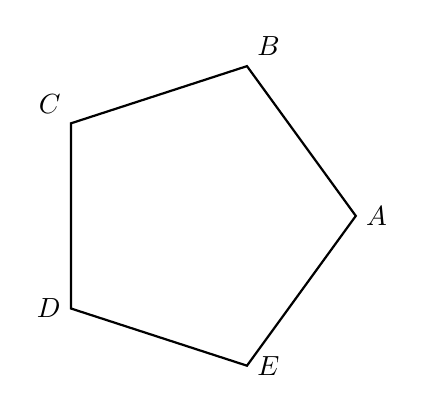
\begin{tikzpicture}%[scale=.48]
         \draw [thick]
         (0:2) node[right] {$A$}--
         (72:2) node[above right] {$B$}--
         (144:2) node[above left] {$C$} --
         (216:2) node[left] {$D$}--
         (288:2) node[right] {$E$}--cycle;
       \end{tikzpicture}
     \end{center}



    \item The vertices of $\triangle JKL$ have the coordinates $J(-4,-2)$, $K(4,2)$, and $L(-2,4)$, as shown. \\[0.25cm]
    Apply a dilation to $\triangle JKL \rightarrow \triangle J'K'L'$, centered on the origin and with a scale factor $k=1.5$. Draw the image $\triangle J'K'L'$ on the set of axes below, labeling the vertices, and make a table showing the correspondence of both triangles' coordinate pairs.  \vspace{4cm}
    \begin{center}
      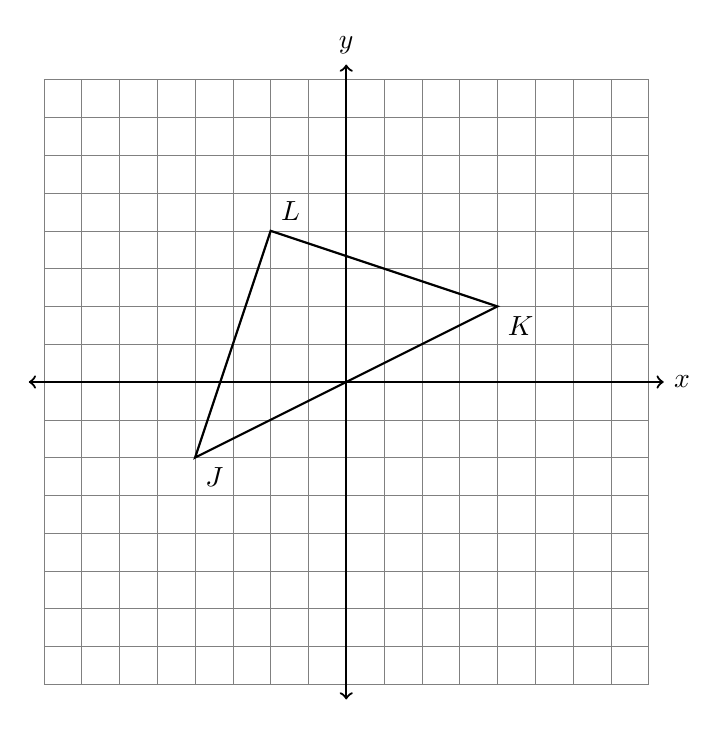
\begin{tikzpicture}[scale=.48]
        \draw [help lines] (-8,-8) grid (8,8);
        \draw [thick, <->] (-8.4,0) -- (8.4,0) node [right] {$x$};
        \draw [thick, <->] (0,-8.4)--(0,8.4) node [above] {$y$};

        \draw [thick]
        (-4,-2) node[below right] {$J$}--
        (4,2) node[below right] {$K$}--
        (-2,4) node[above right] {$L$}--
        cycle;
      \end{tikzpicture}
    \end{center}

\newpage

  \item Triangle $ADE$ and its midline $\overline{BC}$ are drawn, with $B$ the midpoint of $\overline{AD}$ and $C$ the midpoint of $\overline{AE}$. The two medians $\overline{BE}$ and $\overline{CD}$ are drawn, as shown, intersecting in point $F$, the centroid.\\[0.25cm]
  $\triangle FCB \sim \triangle FDE$ with scale factor $k=2$.\\[0.25cm]
  Given $BC=7$, find $DE$. \\[0.25cm] Given $BF=3$, find $FE$. %\vspace{1cm}
  \begin{center}
      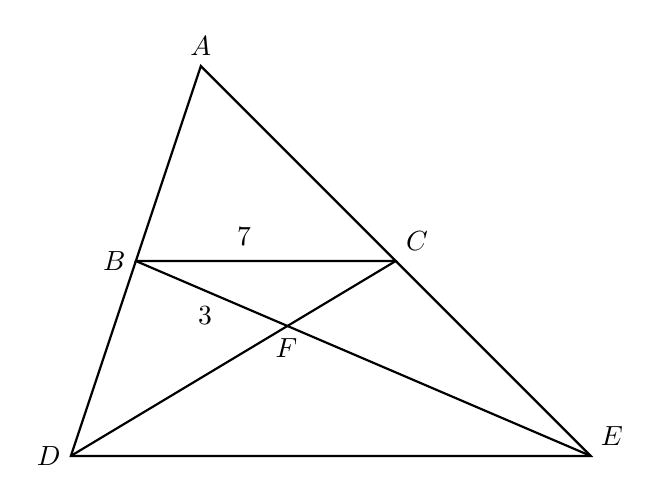
\begin{tikzpicture}[scale=0.55]
        \draw [thick]
        (0.5,1.5)node[left]{$B$}--
        (6.5,1.5)node[above right]{$C$}--
        (2,6)node[above]{$A$}--cycle;
        \draw [thick]
        (0.5,1.5)--
        (-1,-3)node[left]{$D$}--
        (11,-3)node[above right]{$E$}--(6.5,1.5);
        \draw [thick] (0.5,1.5)--(11,-3);
        \draw [thick] (6.5,1.5)--(-1,-3);
        \node at (3,2.5)[below]{$7$};
        \node at (3.5, -0.5)[right]{$F$};
        \node at (2.1, -0.2)[above]{$3$};
        %\node at (-0.7, -1)[above]{$5$};
      \end{tikzpicture}
    \end{center} \vspace{1cm}

 \item Determine and state the transformation or sequence of transformations  applied to $\triangle ABC$, mapping it onto $\triangle PQR$, as shown.
   \begin{center}
       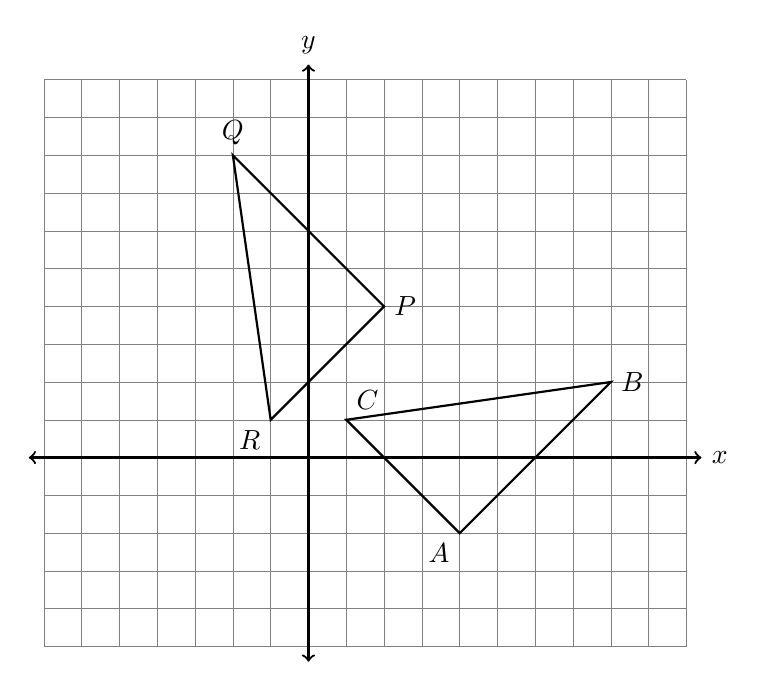
\begin{tikzpicture}[scale=.48]
         \draw [help lines] (-7,-5) grid (10,10);
         \draw [thick, <->] (-7.4,0) -- (10.4,0) node [right] {$x$};
         \draw [thick, <->] (0,-5.4)--(0,10.4) node [above] {$y$};

         \draw [thick]
         (4,-2) node[below left] {$A$}--
         (8,2) node[right] {$B$}--
         (1,1) node[above right] {$C$}--cycle;

         \draw [thick]
         (2,4) node[right] {$P$}--
         (-2,8) node[above] {$Q$}--
         (-1,1) node[below left] {$R$}--cycle;
       \end{tikzpicture}
     \end{center}

\newpage
  \item The $\triangle ABC$ is reflected across $l$ to yield $\triangle A'B'C'$. $AB=x+5$, $A'B'=2x-1$, and $BC=3x+2$. Find the length $B'C'$. %\vspace{2cm}
      \begin{center}
      \begin{tikzpicture}[scale=.8]
        \draw [dashed, <->] (-1,-1)--(7,7) node[below right]{$l$};
        \draw [thick]
        (5,-1) node[below right] {$A$}--
        (8,2) node[right] {$B$}--
        (1,0) node[below left] {$C$}--cycle;
        \draw [thick]
        (-1,5) node[left] {$A'$}--
        (2,8) node[below right] {$B'$}--
        (0,1) node[below left] {$C'$}--cycle;
      \end{tikzpicture}
    \end{center} \vspace{2cm}

  \item In the diagram below, the chords $\overline{AE}$ and $\overline{BD}$ intersect at $C$. Given that $\triangle ABC \sim \triangle DEC$, $AB=2$, $DE=4$, and $AC=3$. Determine the length of $\overline{CD}$.
      \begin{center}
      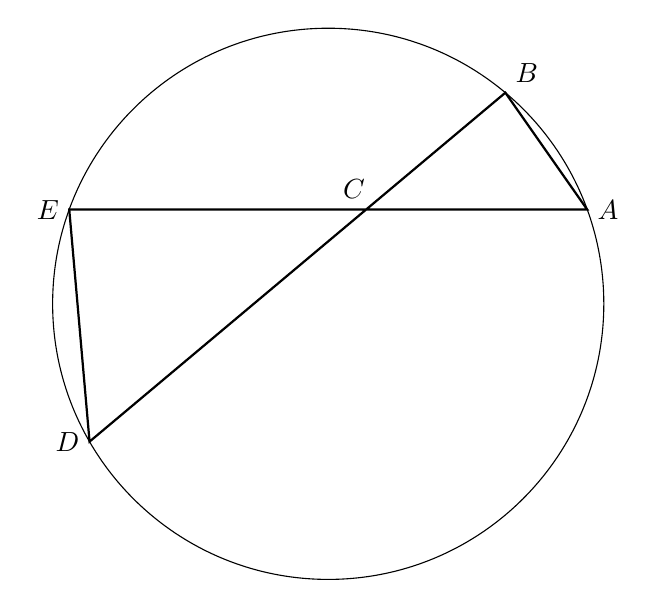
\begin{tikzpicture}[scale=.7]
        \draw (0,0) circle[radius=5];
        \draw [thick]
        (20:5) node[right] {$A$}--
        (160:5) node[left] {$E$}--
        (210:5) node[left] {$D$}--
        (50:5) node[above right] {$B$}--cycle;
        \draw (75:1.8) node[above] {$C$};
      \end{tikzpicture}
    \end{center}

\newpage


  \item In the diagram below, $\triangle ABC \sim \triangle DEF$, $DE=4$, $AB=x$, $AC=x+2$, and $DF=x+6$. Determine the length of $\overline{AB}$.\\[0.5cm]
    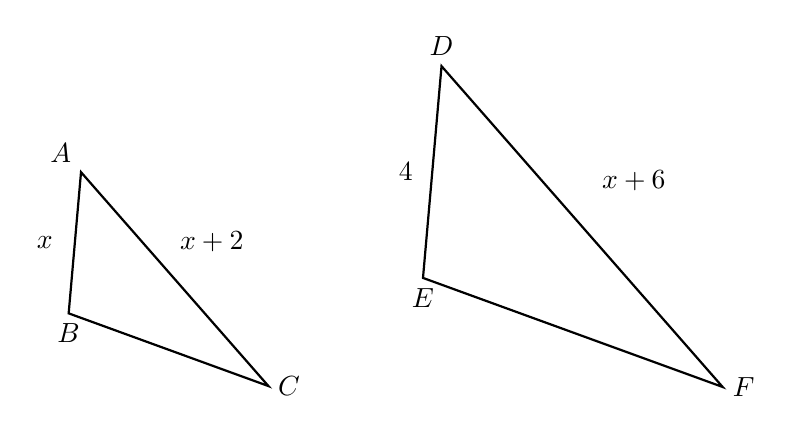
\begin{tikzpicture}[scale=0.9]
      \coordinate [label=above left:$A$](A) at (85:2);
      \coordinate [label=below:$B$](B) at (0, 0);
      \coordinate [label=right:$C$](C) at (-20:3);
        \draw [thick] (A)--(B)--(C)--cycle;
        \node at (95:1)[left]{$x$};
        \node at (35:1.75)[right]{$x+2$};
        \draw [thick, xshift=5cm, yshift=0.5cm] (85:3) node[above]{$D$}--
        (0,0) node[below]{$E$}--
        (-20:4.5) node[right]{$F$}--cycle;
        \draw [thick, xshift=5cm, yshift=0.5cm](90:1.5) node[left]{$4$};
        \draw [thick, xshift=5cm, yshift=0.5cm](30:2.75) node[right]{$x+6$};
    \end{tikzpicture}

\vspace{2cm}

  \item In the diagram below, the chords $\overline{AE}$ and $\overline{BD}$ intersect at $C$. Given that $\triangle ABC \sim \triangle DEC$, $AB=2$, $DE=4$, and $AC=3$. Determine the length of $\overline{CD}$.
      \begin{center}
      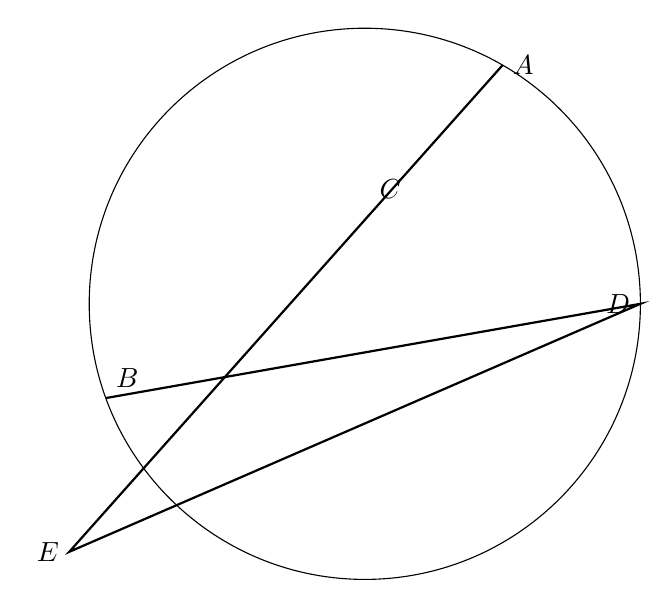
\begin{tikzpicture}[scale=.7]
        \draw (0,0) circle[radius=5];
        \draw [thick]
        (60:5) node[right] {$A$}--
        (220:7) node[left] {$E$}--
        (0:5) node[left] {$D$}--
        (200:5) node[above right] {$B$};
        \draw (75:1.8) node[above] {$C$};
      \end{tikzpicture}
    \end{center}


    \item Given $\triangle ABP$ and $\triangle JKP$ as shown below. $\overline{AB} \parallel \overline{JK}$ with $AB=5$, $PA=4$, $PB=2$, and $PK=5$.\\[0.25cm]
    Find $PJ$ and $JK$.\\[0.5cm]
      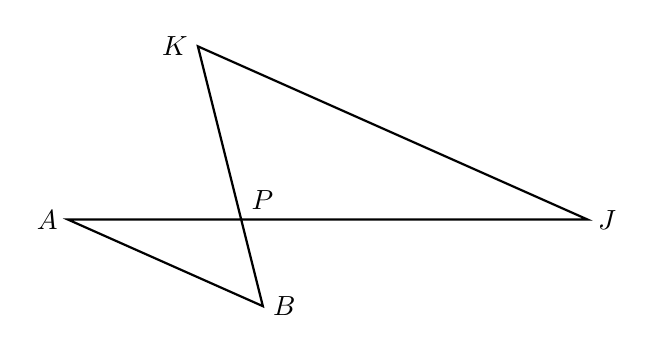
\begin{tikzpicture}[scale=1.1]
          \draw [thick]
            (0.25,-1)node[right]{$B$}--
            (-0.5,2)node[left]{$K$}--
            (4,0)node[right]{$J$}--
            (0,0)node[above right]{$P$}--
            (-2,0)node[left]{$A$}--cycle;
        \end{tikzpicture}
        \vspace{3cm}


\end{enumerate}
\end{document}
